\documentclass[10pt]{article}
%\usepackage{anysize}
%\papersize{11in}{8.5in}
%\marginsize{1in}{1in}{.5in}{.5in}
\textwidth = 6.5 in
\textheight = 9 in
\oddsidemargin = 0.0 in
\evensidemargin = 0.0 in
\topmargin = -0.5 in
\headheight = 0.35 in
\headsep = 0.15 in
\topskip = 0 in
\footskip = 0.5 in
\pagenumbering{arabic}
\usepackage{setspace}
\usepackage[usenames]{color}
\usepackage[fleqn]{amsmath}
\usepackage{graphicx}
\usepackage{url}
\usepackage{verbatim}
\usepackage{indentfirst}
\usepackage{booktabs}
\usepackage{multirow}
\usepackage[table]{xcolor}
\usepackage{ragged2e}
\usepackage{xspace}
\usepackage{parskip}
\usepackage{tabulary}
\usepackage[normalem]{ulem}
\usepackage{hyperref}
\hypersetup{pdfborder={0 0 0}, colorlinks=true, urlcolor=blue, linkcolor=black}
\usepackage[format=plain, labelsep=period, justification=raggedright, singlelinecheck=true, skip=2pt, font={footnotesize,sf}, labelfont=bf]{caption}
\usepackage{titlesec}
\usepackage{lastpage}
\usepackage{fancyhdr}
\usepackage{ifthen}
\usepackage{wrapfig}

%\usepackage[round]{natbib}
%\bibliographystyle{evolution}
\usepackage[style=nature]{biblatex}
\bibliography{references}

%% Format headers and footers %%%%%%%%%%%%%%%%%%%%
\pagestyle{fancy}
%\lhead{\ifthenelse{\value{page}=1}{}{\sffamily\footnotesize Jamie Oaks}}
\lhead{\sffamily \emph{\docTitle} \\ Jamie R. Oaks}
%\chead{\ifthenelse{\value{page}=1}{{\scshape \docTitle} \\ Jamie Richard Oaks}{\sffamily\footnotesize \docTitle}}
%\rhead{\ifthenelse{\value{page}=1}{}{\sffamily\footnotesize \today}}
\rhead{\sffamily \today}
\cfoot{\sffamily\footnotesize Page \thepage\ of \pageref{LastPage}}
\renewcommand{\headrulewidth}{0.4pt}
\renewcommand{\footrulewidth}{0pt}

%% Format section titles %%%%%%%%%%%%%%%%%%%%%%%%%
\renewcommand\refname{Peer-reviewed Publications}

\titleformat{\section}[hang]
    {\large\sffamily\bfseries}
    {\S\ \thesection.}{.5em}{}[]
\titlespacing{\section}
    {0mm}{1.0ex plus .1ex minus .1ex}{-0.5ex}

\titleformat{\subsection}[hang]
    {\large\sffamily\itshape}
    {\S\ \thesection.}{.5em}{}[]
\titlespacing{\subsection}
    {0mm}{1.0ex plus .1ex minus .1ex}{-0.5ex}

\titleformat{\subsubsection}[runin]
    {\sffamily\bfseries}
    {\S\ \thesection.}{.5em}{}[.---]
\titlespacing{\subsubsection}
    {\parindent}{0pt}{0pt}
%    {\parindent}{1.0ex plus .1ex minus .1ex}{0pt}

%% Format list environments %%%%%%%%%%%%%%%%%%%%%%%%
\renewcommand{\labelenumii}{\arabic{enumi}.\arabic{enumii}}
\renewcommand{\labelitemi}{$\circ$}

\newenvironment{myEnumerate}{
  \begin{enumerate}
    \setlength{\itemsep}{0.25em}
    \setlength{\parskip}{0pt}
    \setlength{\parsep}{0.5em}}
  {\end{enumerate}}

\newenvironment{myItemize}{
  \begin{itemize}
    \setlength{\leftskip}{-4mm}
    \setlength{\itemsep}{0.25em}
    \setlength{\parskip}{0pt}
    \setlength{\parsep}{0.5em}}
  {\end{itemize}}

%% Basic formatting and spacing %%%%%%%%%%%%%%%%%%%%%
\setlength{\parindent}{0em}
\setlength{\parskip}{0.5em}

%% My functions %%%%%%%%%%%%%%%%%%%%%%%%%%%%%
\newcommand{\ignore}[1]{}
\newcommand{\addTail}[1]{\textit{#1}.---}
\newcommand{\super}[1]{\ensuremath{^{\textrm{#1}}}}
\newcommand{\sub}[1]{\ensuremath{_{\textrm{#1}}}}
\newcommand{\dC}{\ensuremath{^\circ{\textrm{C}}}}
\newcommand{\tableSubItem}{\addtolength{\leftskip}{1em} \labelitemi \xspace}
\newcommand{\myHangIndent}{\hangindent=5mm}

%%%%%%%%%%%%%%%%%%%%%%%%%%%%%%%%%%%%%%%%%%%%%%%%%%%%%%%%%%%%%%
%%%%%%%%%%%%%%%%%%%%%%%%%%%%%%%%%%%%%%%%%%%%%%%%%%%%%%%%%%%%%%
\newcommand{\docTitle}{Research Statement\xspace}
\begin{document}
\raggedright
\singlespacing

\textbf{\textit{What historical and ecological processes shape genetic variation both temporally and spatially, partition evolutionary lineages, and generate and maintain biodiversity?}} \\
Elucidating the answers to this question is the primary motivation of my research program.
To address this question, I use patterns of DNA sequence variation within and among species to identify independent evolutionary lineages (i.e., species) and infer their demographic histories and relationships, testing for patterns predicted by current ecological factors and historical events.
To do this as robustly as possible, my research also strongly focuses on the development, implementation, and application of phylogenetic and phylogeographic models of evolution.

\section*{Previous \& Current Research}
%%%%%%%%%%%%%%%%%%%%%
\subsection*{Diversification of Crocodiles}
Traditionally, crocodiles (\emph{Crocodylus}) have been stereotyped as an ancient group of ``living fossils'' that originated in Africa prior to the fragmentation of Pangea; their diversity and circumtropical distribution was attributed to vicariance via continental drift.
However, early molecular data and subsequent reassessment of paleontological data suggested the genus could be younger than previously believed.
Recently, I collected a large multi-locus dataset of all extant crocodylian species and used novel statistical phylogenetic methods to infer the temporal and biogeographical origin of \emph{Crocodylus}.
My results overturned traditional views of crocodiles as ``living-fossils'' from Africa, revealing a recent and dynamic evolutionary history \footfullcite{Oaks2011}.
My results strongly support that all extant crocodiles shared a common ancestor from the tropics of the Indo-Pacific, approximately 14--8 million years ago (mya), rejecting an ancient vicariant explanation of their biogeography in favor of a recent, dispersal-mediated model involving multiple transoceanic dispersals.
It was not until after the mid-Miocene climatic optimum, when the global climate was cooling and fellow crocodylian lineages were suffering massive extinctions, that \emph{Crocodylus} radiated and dispersed around the globe.
This finding suggests it was not only global cooling driving the extinction of other crocodylians, as previously believed, but also most likely competition with the rapidly radiating \emph{Crocodylus} lineage.
%My results also revealed more species diversity within the \emph{Crocodylus} than currently recognized.

This study also introduced important methodological innovations.
To accommodate the variation of substitution rates among DNA sites in the alignment, I used a novel approach of estimating the optimal model for partitioning the alignment.
The resulting models performed far better than traditional models that partition based on \emph{a priori} expectations \footfullcite{OaksInPrep}.
This has important implications, because improved modeling of among-site rate variation will mitigate the underestimation of long branches and concomitant systematic error in phylogenetic estimates (e.g., long-branch attraction).
Furthermore, the estimated phylogeny was among the first time-calibrated species tree inferred under a multi-species coalescent model, and was the first to use a posterior sample of species trees to estimate ancestral-state reconstructions.
The species trees represent direct estimates of the evolutionary history of the species, rather than a proxy estimate of the history of individual gene copies.
A direct representation of the species tree is ideal when inferring the evolutionary patterns of species-level characters, like ancestral ranges.

\subsection*{Climate-Driven Diversification}
The main focus of my current research seeks to determine whether Quaternary climatic oscillations promoted diversification by fragmenting the distributions of species.
An ideal model system for such research exists in the complex system of island archipelagos in Southeast Asia.
The Southeast Asian mainland and complex system of 26,000+ islands experienced dramatic cyclical shifts in the extent of the terrestrial landscape during Quaternary glacial cycles (Figure \ref{map}).
Many groups of islands in this region coalesced into aggregated islands during glacial periods when sea levels were up to 120m below current level; these aggregated islands where repeatedly fragmented during interglacial highstands.

The repeated formation and fragmentation of these Pleistocene aggregate island complexes (PAICs) has been best characterized in the 7100+ islands of the Philippines, where it has become a prominent paradigm for understanding the biodiversity of the archipelago.
The PAIC model has most commonly been used to delineate areas of endemism across the Philippines, but has also been hypothesized to have increased the biodiversity of the islands by promoting speciation during island fragmentation.
To assess the validity of the PAIC model of diversification, collaborators and I have been studying the evolutionary history of two genera of geckos (\emph{Cyrtodactylus} and \emph{Gekko}) that are co-distributed across most of the islands of the Philippines\footfullcite{Siler2010}\super{,}\footfullcite{Siler2012}.
We found that PAIC islands did explain a significant proportion of the genetic diversity, but populations from PAICs were not monophyletic, and there was no obvious pattern of diversification associated with the Pleistocene.
We revealed complex histories for both genera that contradict many of the the traditional PAIC model predictions.
Interestingly, for \emph{Gekko}, we found evidence that the genus colonized the Philippines by ``rafting'' on the Palawan Microcontinental Islands that rifted away from Mainland Asia and drifted towards the rest of the Philippine Archipelago between 30--10 mya.

\begin{wrapfigure}{r}{0.54\textwidth}
  \vspace{-1.5em}
  \begin{center}
    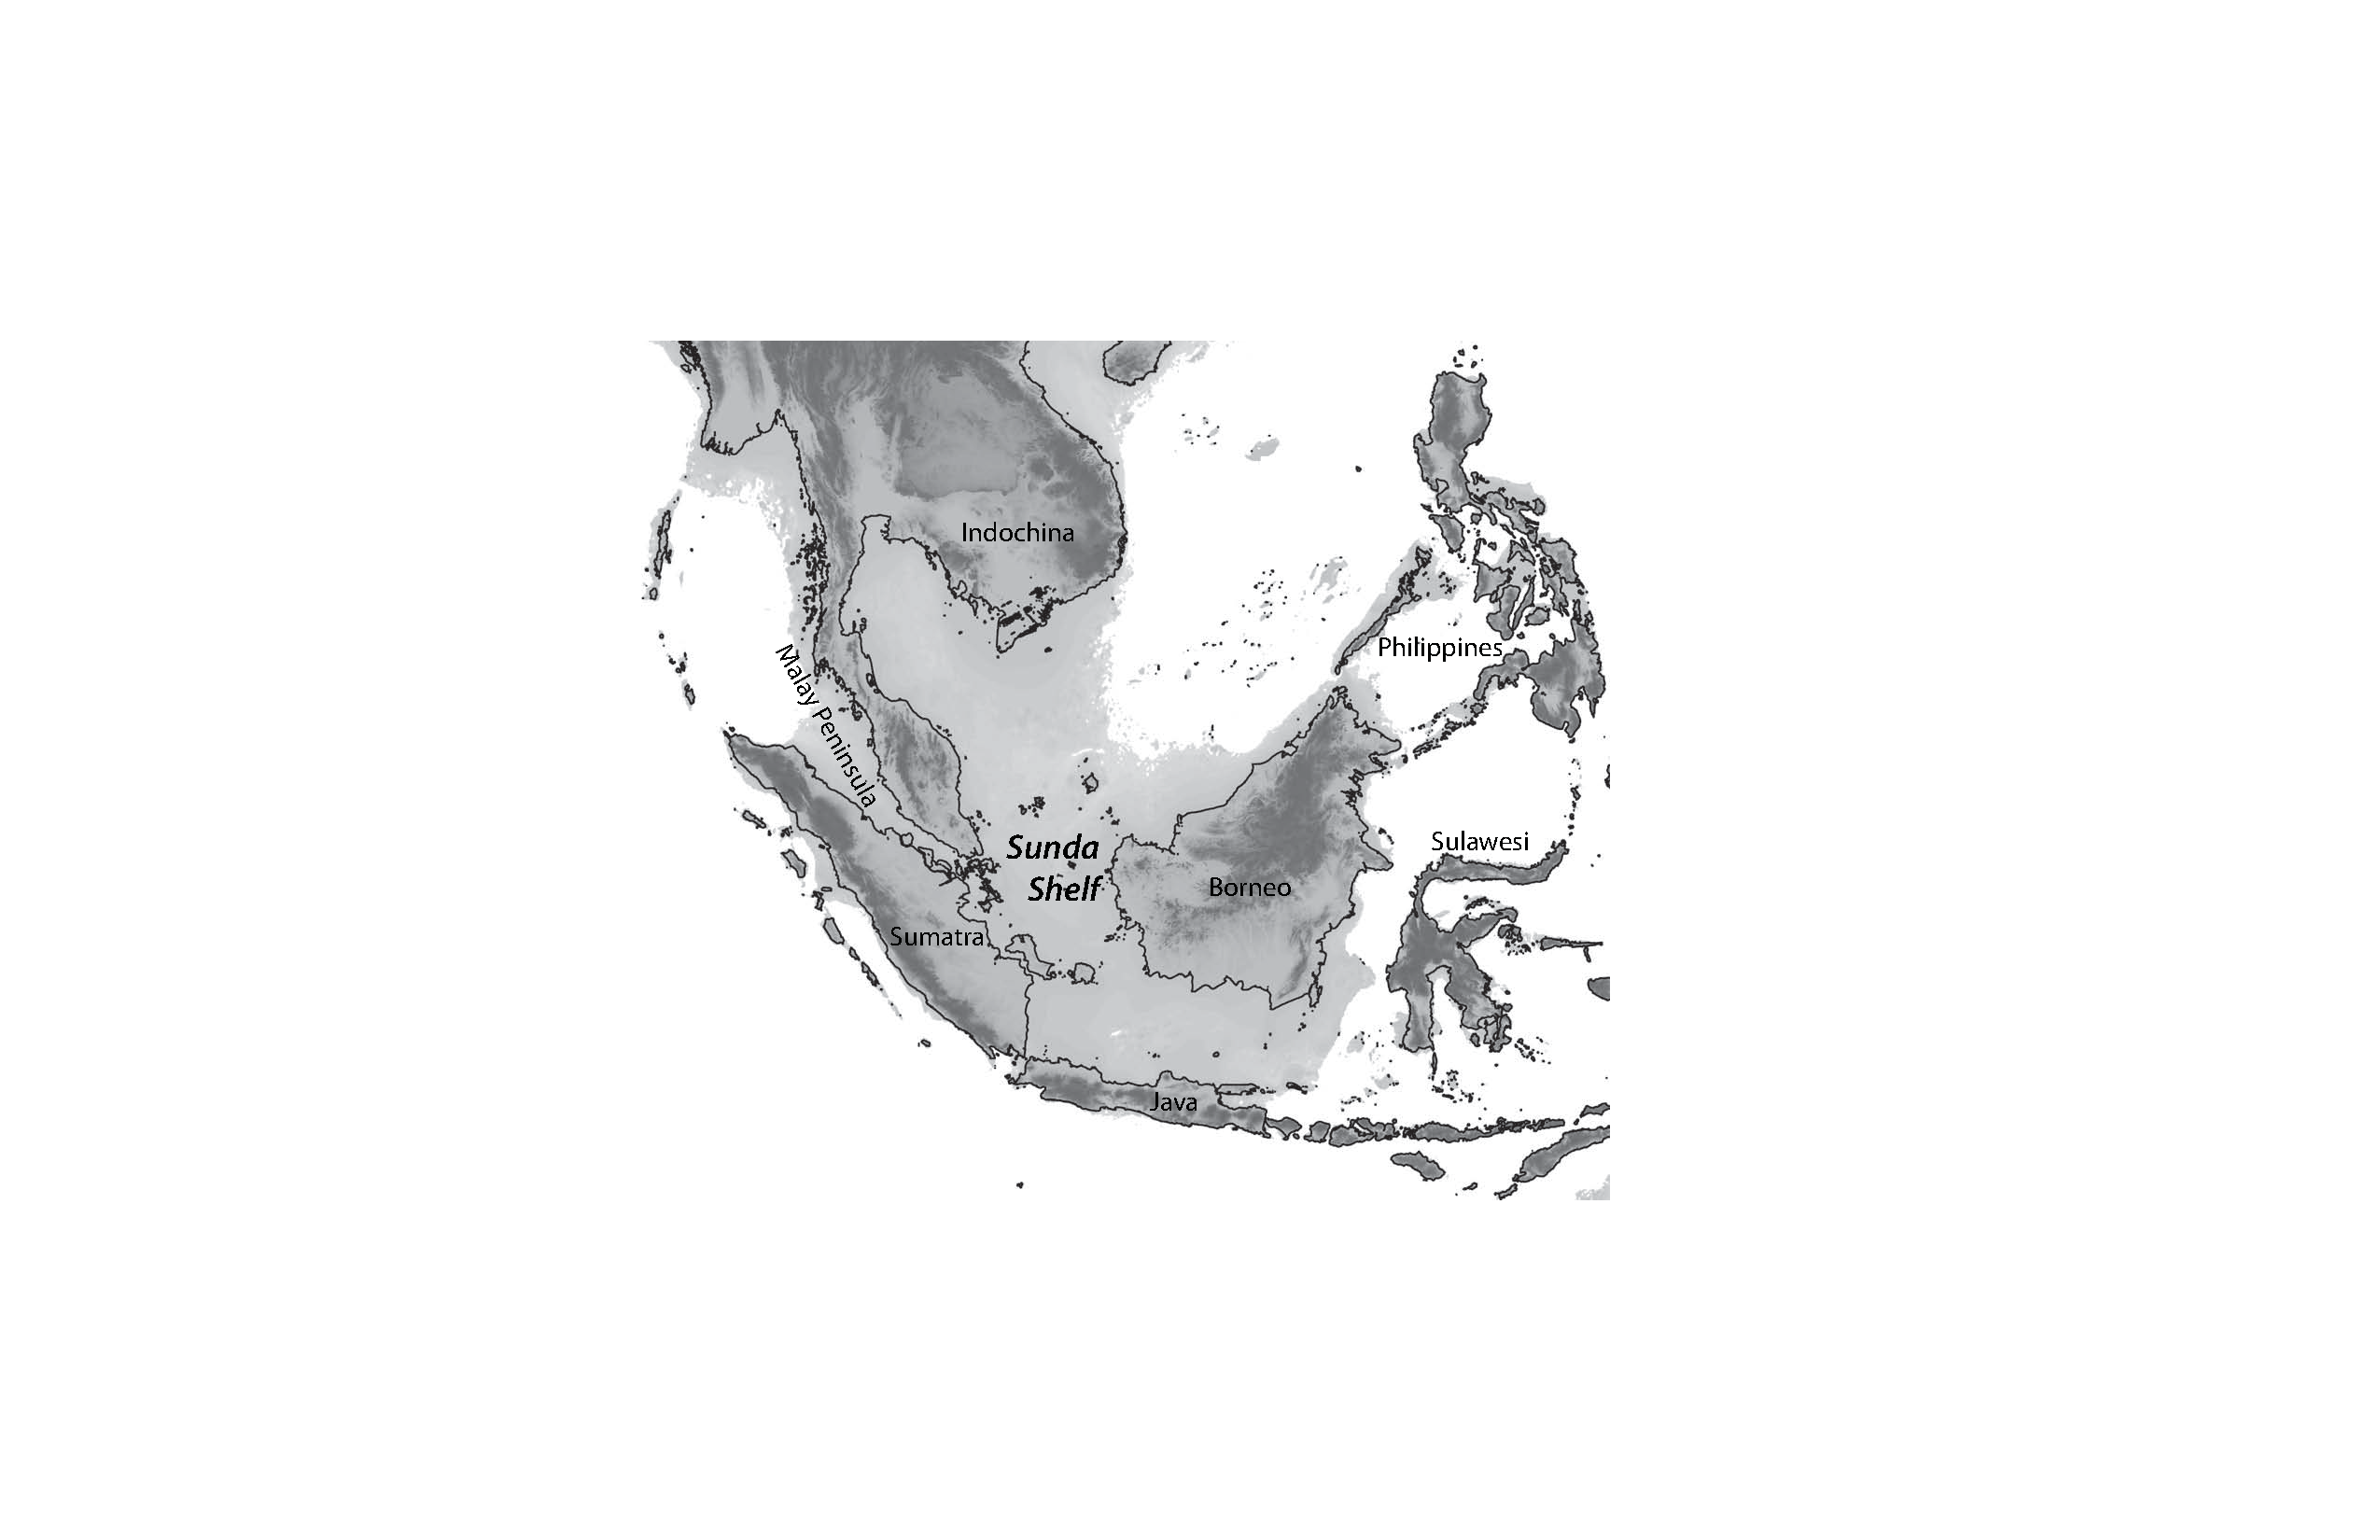
\includegraphics[width=0.53\textwidth]{sunda_shelf_small.pdf}
  \end{center}
  \vspace{-0.2em}
  \caption{Map of Southeast Asia with land extent (depicted in grey) during glacial lowstands estimated using 120m bathymetry (data from \href{http://ngdc.noaa.gov/mgg/global/global.html}{ETOPO1}).}
  \label{map}
  \vspace{-1.1em}
\end{wrapfigure}

Recognizing that the shallow timescale of the PAIC cycles is not necessarily conducive for traditional phylogenetic investigations, we also addressed the PAIC diversification hypothesis using a comparative, coalescent-based approach \footfullcite{Oaks2012}.
If repeated bouts of island connectivity and isolation promoted diversification, the temporal distribution of divergences between inter-island populations within PAICs should be temporally clustered and correspond with interglacial rises in sea level.
To test this prediction, we accumulated genetic data from 22 distantly related pairs of populations, representing five orders of terrestrial vertebrates.
Each pair of populations is currently on two separate islands that were historically connected during glacial periods.
We inferred the distribution of divergence times across the 22 pairs of populations using a popular approximate Bayesian computation (ABC) method implemented in a software package called msBayes.
We found very strong support (posterior probability of 0.982) for a recent, simultaneous divergence event shared by all 22 taxa.

Rather than interpret this support for simultaneous divergence across the 22 taxa as strong evidence of climate-driven diversification, I performed extensive simulation-based analyses to assess the ability of the msBayes method to detect variation in divergence times.
The results of the simulations revealed that msBayes has low power and is biased towards inferring ``simultaneous'' divergence; I demonstrated that we were likely to have inferred simultaneous divergence even if the 22 population pairs had randomly diverged over the past 3--2 million years.
This finding is important, because msBayes is a popular method, and inferences of clustered divergence times across co-distributed taxa has often been interpreted as evidence for a shared historical event in the literature.
Our results demonstrate that the method can be biased towards such results, and the interpretation of a shared event is not warranted without simulation-based validation of the method's performance.

Given that we have exhausted currently available methods using moderate-sized datasets, I am currently using an integrative approach to better assess the Pleistocene-diversification hypothesis.  Concurrently, I am (1) collecting genome-scale data from dense sampling of \emph{Cyrtodactylus} and \emph{Gekko} from across the Philippine Archipelago using next-generation sequencing technology, and (2) implementing a more powerful, comparative phylogeographic method for inferring the temporal distribution of divergences within a fully Bayesian multi-species coalescent framework.

\subsubsection*{1) Next-generation sequencing of geckos}
I am currently collecting genomic sequence data at low-level coverage from a small subset of our \emph{Cyrtodactylus} and \emph{Gekko} samples using Illumina TruSeq SBS sequencing chemistry.
The goal is to use the resulting genomic data to design probes for 200 effectively unlinked, single-copy loci from across the genome to allow enrichment of these targets for next-gen sequencing across all the samples.
Collecting hundreds of unlinked loci will give us much more power to infer demographic parameters using coalescent-based methods.

\subsubsection*{2) Implementing a fully Bayesian comparative phylogeographic model}
The evolutionary genetics software package, BEAST (\url{http://code.google.com/p/beast-mcmc/}), implements a Bayesian multi-species coalescent model that jointly estimates multiple gene trees and the shared species tree in which they evolve.
In this model, the divergence times (node heights of the rooted, ultrametric species tree) are among the parameters that are jointly estimated.
As a developer for BEAST, I am working on a reversible-jump Markov chain Monte Carlo (MCMC) method that will co-estimate the number of divergence ``events'' represented across the species tree, the timing of them, and the assignment of nodes to the divergence events, all while integrating over uncertainty in the substitution and coalescent processes, gene trees, and species tree.
The goal is to be able to infer the pattern of divergence times across a species tree, and test whether certain divergences are more clustered then expected by chance.

This model will have several advantages over the ABC method of msBayes.
It will take advantage of the full information in the sequence data by estimating the posterior probability distributions of the model parameters directly from the sequence data, avoiding the loss of information suffered by ABC when distilling the data into summary statistics.
The new method will estimate the relative mutation rates across the species tree using rigorous relaxed-clock models already implemented in BEAST.
This will provide more accurate estimates of species divergence than msBayes, which assumes mutation rates are equal across taxa.
Also, by using a fully phylogenetic framework, we can infer more complicated patterns of divergence times than is possible with msBayes, which is restricted to comparing pairs of taxa.

\section*{Future Research}
%%%%%%%%%%%%%%%
\subsection*{Simultaneous Estimation of Population History and Structure: A Novel Approach}
Currently, the inference of species trees from multi-locus genetic data collected at a phylogeographic scale is typically conducted in a two-step process.
First, the investigator must estimate how many populations (or species) are represented in their sample, and assign individuals to those populations.
This is typically done using some variant of a genetic clustering algorithm.
Second, the relationships among the resulting clusters is then inferred under a multi-species coalescent model.
The reason this two-step process is currently necessary is because current implementations of multi-species coalescent models assume the population assignment is known without error, and is fixed during the analysis.
This assumption is often unrealistic for empirical data, because it is often difficult to diagnose cryptic, independent evolutionary lineages with complete certainty.
Another potential problem with this approach is that the genetic clustering methods simply group individuals based on allele frequencies, and do not use the information contained in the sequence data about the genealogical history of the alleles; using such information is a major strength of coalescent-based methods.
Thus, initially inferring the population assignments using allele-frequency-based methods does not make full use of the sequence data and is more likely to lead to erroneous results.

A more robust approach would be to integrate these two steps and make population assignment a random variable estimated during the inference of the population tree.
I will collaborate with Mark Holder to develop a method to do this using a nonparametric Bayesian MCMC method that treats population assignment as a random variable under a discrete prior distribution.
There are several probability distributions (e.g. Dirichlet process, Pitman-Yor process, and uniform process) commonly used as priors in Bayesian nonparametric statistics in situations such as this, where we need to estimate the assignment of random variables (gene copies) to groups (populations).
We will implement this method by incorporating a Gibbs sampling proposal mechanisms into the BEAST MCMC machinery that numerically integrates over the possible numbers of populations and individual assignments.
%This sampling procedure entails picking a gene copy, removing it from its current population and re-assigning it to one of the other populations or a new population according to probabilities calculated using the likelihood function of the *BEAST model and the current states of other parameters.
%This procedure will be repeated, sweeping across all gene copies, resulting in a newly proposed population structure.
%As with all other proposals, acceptance as the next state in the Markov chain will be governed by the Metropolis-Hastings algorithm.
This software tool will benefit a broad community of researchers conducting phylogeographic analyses, and we plan to propose the project to the NSF Division of Environmental Biology (DEB) Phylogenetic Systematics Program to secure funds for the necessary computational resources.

\subsection*{Diversification and Adaptation of Lizards on Continental Islands of the Sunda Shelf}
The Sunda Shelf of Southeast Asia has been an incredibly dynamic landscape over the past two million years.
The extent of terrestrial habitat has fluctuated dramatically throughout the Quaternary glacial cycles (Figure \ref{map}).
Currently surrounding mainland Southeast Asia and the major islands of the Sunda Shelf, are a network of small continental islands that were formally part of the Sunda Peninsula during glacial periods.
Many of these islands are merely wind-swept rocky outcrops that, nonetheless, support small populations of skinks (\emph{Eutropis multifasciata}) and geckos (\emph{Lepidodactylus lugubris}).
Many of these islands were likely completely inundated during the last two interglacial highstands ($\sim$400,000 and $\sim$120,000 years ago) when sea levels were up to 20+ m above present.
For the next 100,000 years, these islands were part of the exposed Sunda Shelf landmass during the Wisconsin glaciation, before being fragmented by rising sea levels $\sim$12,000 years ago.

The lizard species inhabiting these islands have interesting biologies.
\emph{E.\ multifasciata} has occupied a distinct niche from their mainland, forest-dwelling counterparts; they subsist off arthropods attracted to the debris of nesting colonies of terns.
They also exhibit extreme polymorphisms in color patterns among island populations, far exceeding the variation seen on the mainland.
Furthermore, across its broad range, \emph{E.\ multifasciata} populations vary between egg-laying (oviparity) and live-bearing (ovoviviparity) modes of reproduction.
%\emph{L.\ lugubris} is often restricted to peripheral habitats, such as wind-swept rocky islands, because it is outcompeted by other gecko species in more typical gecko habitats.
Similarly, populations of \emph{L.\ lugubris} also vary in reproductive mode across the range of the species; some population are comprised solely of asexual, parthenogenetic females, whereas others are sexual.

The network of minuscule islands distributed across the Sunda Shelf harboring small insular populations of co-distributed lizards offers a unique model system for studying the 
1) affects of recent, severe fragmentation on historical demography and diversification,
2) evolution of reproductive mode,
3) rapid evolution of color pattern, and 
4) the interplay between selection and genetic drift in extremely small populations under strong selective pressures.
My collaborators and I will foster this natural model system as part of a long-term project to address these questions.
My collaborators include
Dr. Lee Grismer, Professor of Biology at La Sierra University, and international colleagues
Dr. Norhayati Ahmad, Professor of Science and Technology at the Universiti Kebangsaan Malaysia (UKM), and
Dr. Shahrul Anuar Mohd Sah, Professor of the Biological Sciences at the Universiti Sains Malaysia (USM).
We plan to approach different aspects of this study in a series of stages.

The first stage will entail next-gen sequencing of hundreds of loci from dense sampling of individuals of both species across the islands and surrounding landmasses, and collecting a database of whole genomes and transcriptomes from a subset of individuals from a few of the well-sampled islands of known reproductive mode and color phenotype.
With the multi-locus data, we will elucidate the evolutionary context of the island populations by using coalescent-based models to infer their past demography and relationships.
Not only will this address interesting questions about the evolution of populations in this dynamic fragmented landscape, but will also create an evolutionary framework to guide additional data collection and analyses.
It will allow us to appropriately model the genetic covariance among populations in all downstream analyses, avoiding the erroneous assumption of independence among populations.
Using the preliminary genomic and transcriptomic data, we will begin to characterize the genetic underpinnings of the variable natural-history characteristics of both species (reproductive modes and color patterns).
We will determine whether the phenotypic variation for each trait is predominantly the result of variation in coding or regulatory sequences.
We will seek funding from the NSF Phylogenetic Systematics Program for this initial stage of the project.

Once we identify the regions of the genome relevant to the variation in the traits of interest, we will begin the second stage of the project, in which we will collect sequence data from these regions from dense population-level sampling across the islands and neighboring mainland.
This stage will also entail field and lab observations to characterize the traits of interest in each population.
Using these data, we can determine if the genetic variants responsible for the different phenotypes are the result of independent, parallel mutations, or whether these variants are present across much of the distribution of these species at low frequencies and are independently fixed among different populations.
We will also analyze these data within the phylogeographic context of the populations elucidated in Stage 1 to understand the relative contributions of selection versus drift in the evolution of these traits.
These populations have recently been restricted to the unusual, harsh habitats of the Sunda Shelf islands and have likely been experiencing strong selective pressures as a result.
At the same time, genetic drift is undoubtedly an extremely strong evolutionary force on these islands where populations consist of only tens to hundreds of breeding adults.
This offers a natural model system for studying the interplay between the deterministic force of selection and the stochastic force of drift in shaping the genomic landscapes and phenotypic characteristics of these populations.
We will seek funding from the NSF Phylogenetic Evolutionary Genetics Program for the second stage of the project.

Once we have established the phylogeographic context of the island populations and the genetic mechanisms responsible for their phenotypic variation, the third stage of the project will aim to understand the evolutionary ecology of this system.
We want to understand what intra-specific, inter-specific, and abiotic interactions influence the selection on the regions of the genome that control important phenotypic characteristics.
For example, are there particular ecological contexts that favor parthenogenesis in \emph{L.\ lugubris}?
Are there particular inter-specific interactions that favor ovoviviparity in \emph{E.\ multifasciata}, like introduced mammalian predators of lizard eggs?
Are the striking color polymorphisms of \emph{E.\ multifasciata} adaptive?
From the fieldwork and sequence collection associated with the first to stages of this project, we hope to sufficiently characterize the ecosystems of these islands and have the necessary genomic data to allow us to assess such questions at the genetic level in these species.
We feel this third stage will be a strong candidate for the NSF Evolutionary Ecology Program.

\end{document}
%%%%%%%%%%%%%%%%%%%%%%%%%%%%%%%%%%%%%%%%%%%%%%%%%%%%%%%%%%%%%%
%%%%%%%%%%%%%%%%%%%%%%%%%%%%%%%%%%%%%%%%%%%%%%%%%%%%%%%%%%%%%%
